\documentclass[11pt,a4paper]{article}
\usepackage[margin=1.9cm,top=1.7cm,bottom=1.7cm]{geometry}
\usepackage{fontspec}
\setmainfont{TeX Gyre Termes}
\setmonofont[Scale=0.88]{DejaVu Sans Mono}
\hyphenpenalty=10000\exhyphenpenalty=10000\emergencystretch=3em
\renewcommand{\figurename}{Figura}\renewcommand{\tablename}{Tabela}
\usepackage{microtype,booktabs,graphicx,float,xcolor,enumitem,array,tabularx,caption,titlesec}
\usepackage[hidelinks]{hyperref}
\captionsetup{font=small,labelfont=bf,skip=3pt}
\setlength{\parskip}{2.5pt}\setlength{\parindent}{1.1em}
\setlist{nosep,leftmargin=1.3em}
\titleformat{\section}{\large\bfseries}{\thesection}{.5em}{}
\titleformat{\subsection}{\normalsize\bfseries}{\thesubsection}{.5em}{}
\titlespacing*{\section}{0pt}{7pt}{3pt}
\titlespacing*{\subsection}{0pt}{5pt}{2pt}
\renewcommand{\arraystretch}{1.08}
\newcommand{\us}{\ensuremath{\,\mu\mathrm{s}}}
\begin{document}
\thispagestyle{empty}
\begin{center}
{\large\bfseries UNIVERSIDADE DO VALE DO ITAJAÍ --- UNIVALI}\\
Escola Politécnica --- Engenharia de Computação --- Sistemas em Tempo Real\\[5pt]
{\Large\bfseries Quanto o teste enxerga do pior caso?}\\
{\large Tempo de resposta, HWM e (m,k)-firme da codificação de Huffman em um ESP32}\\[4pt]
Lucas Siqueira Maia (RA: 8319456) \quad Melkior Gabriel Paim Misiak (RA: 8309000)\\
Itajaí, 2026 \quad|\quad Repositório: \texttt{[https://github.com/MelkiorMisiak/str_m3_esp32]}
\end{center}
\vspace{-4pt}

\section{Introdução e plataforma}
Este trabalho mede o tempo de resposta da mesma tarefa, a codificação de Huffman, em quatro escopos de teste com estresse crescente (tarefa, comportamental, intertarefas e sistema), para responder: \emph{se a cobertura de código chega a 100\%, por que o HWM continua crescente? E, quando o WCRT não é alcançável, como o modelo (m,k)-firme transforma as medições em um critério testável?} Todos os números abaixo vêm dos CSV \texttt{etapa1..4.csv} (27\,000 ativações) e do script \texttt{analysis/analyze.py} do repositório, mais o script complementar \texttt{relatorio\_analise.py} (figuras e Experimento D).

\begin{table}[H]\centering\small
\begin{tabularx}{\linewidth}{@{}lX@{}}
\toprule
\textbf{Item} & \textbf{Configuração registrada}\\\midrule
Plataforma & ESP32 (2 núcleos Xtensa LX6) a 240\,MHz fixos; ESP-IDF v6.1-dev com FreeRTOS SMP; tick de 1\,kHz; \texttt{-O2}.\\
Governor de energia & Nenhum: \texttt{CONFIG\_PM\_ENABLE=n} (sem DFS e sem light sleep), frequência constante.\\
Programas em execução & Somente \emph{idle}, \texttt{esp\_timer} e o firmware de teste (sem Wi-Fi/Bluetooth). Tarefas de tempo real fixadas no núcleo 0; a carga da etapa 4 usa também o núcleo 1.\\
Tarefa sob teste & Huffman sem \texttt{malloc}; \textbf{array de 2048 bytes}, gerador xorshift32 com \textbf{semente 123456789}, novo array a cada ativação (fora da janela cronometrada). Valida a saída: decodifica e compara com a entrada (\texttt{huff\_fail=0} nas 27\,000 ativações).\\
Instrumentação & \texttt{clock\_gettime(CLOCK\_MONOTONIC)}, resolução de 1\,\textmu s. Nas etapas 2--4 a liberação é carimbada na ISR do timer (\texttt{esp\_timer}); o desvio de origem entre os dois relógios (73\,130\,\textmu s) foi medido na inicialização e subtraído. Os CSV só são enviados pela serial (921\,600\,baud) \emph{depois} de cada etapa.\\
Ativações & 10\,000 / 2\,000 / 5\,000 / 10\,000 (etapas 1--4); a etapa 4 serve ao Experimento B.\\\bottomrule
\end{tabularx}
\end{table}

\section{Metodologia}
\textbf{Métrica.} Etapa 1: tempo de execução da função (como no exemplo da aula). Etapas 2--4: tempo de resposta = conclusão $-$ liberação, com a liberação marcada na ISR, de modo que o valor inclui latência de interrupção, preempção, bloqueio em mutex e execução.

\textbf{Deadline fixo.} $D=\lceil 1{,}2\times \mathrm{HWM}_{100\%}^{(1)}\rceil=\lceil 1{,}2\times 6371\rceil=\mathbf{7646\us}$, definido uma única vez na etapa 1 e usado nas quatro etapas. A folga de 20\% é a regra prática do enunciado; ela é pequena de propósito, para que o efeito do escopo apareça. Só o Experimento D varia $D$.

\begin{table}[H]\centering\footnotesize
\begin{tabularx}{\linewidth}{@{}p{1.65cm}XXX@{}}
\toprule
\textbf{Etapa} & \textbf{Caso de teste (entradas, restrições, esperado)} & \textbf{Procedimento} & \textbf{Critério}\\\midrule
1 Tarefa & 2048 bytes aleatórios novos a cada ativação; sistema ocioso (espera de 5\,ms entre ativações). Esperado: decodificação = entrada. & Tarefa isolada: \texttt{clock\_gettime} $\to$ codifica+decodifica+compara $\to$ \texttt{clock\_gettime}; 10\,000 ativações. & Validação 100\% correta; HWM(100\%) define $D$.\\
2 Compor\-tamental & Um evento externo por vez: timer de hardware a cada 10\,ms (maior que a execução, sem sobreposição). & A ISR carimba o instante e acorda a Huffman; resposta = fim $-$ carimbo; 2\,000 eventos. & Resposta $\le D$; mede latência de ISR e escalonamento.\\
3 Inter\-tarefas & \emph{sensor} (prio.\,7, 7\,ms), \emph{logger} (prio.\,6, 13\,ms), Huffman (prio.\,5, 20\,ms); mutex com herança de prioridade sobre um buffer de 64\,B (sensor escreve, logger lê, Huffman copia); taxas diferentes e coprimas. & Os três timers são armados juntos (instante crítico em $t=0$, repetido a cada $\mathrm{mmc}(7,13,20)=1820$\,ms); mede-se a Huffman, 5\,000 ativações. & Resposta $\le D$; quantificar perdas, $S$ e (m,k).\\
4 Sistema & Etapa 3 mais carga externa (abaixo). & Idem etapa 3, 10\,000 ativações. & Tentar fazer o sistema perder o prazo; reportar $S$ e (m,k).\\\bottomrule
\end{tabularx}
\end{table}
\textbf{Estresse da etapa 4 (justificativa).} O pior caso de um STR nasce da concorrência de hardware e de interrupções, não de caminhos de código; por isso a carga ataca recursos distintos: (i)~\emph{tempestade de interrupções}, ISR de 40\,\textmu s a cada 700\,\textmu s no núcleo 0 ($\approx$6\% da CPU), que rouba tempo até da tarefa mais prioritária; (ii)~\emph{tráfego de memória}, tarefa no núcleo 1 varrendo 128\,KB de flash e copiando 32\,KB de RAM, que disputa cache e barramento SPI com o núcleo 0; (iii)~\emph{rajadas de CPU}, tarefa de prioridade 6 (acima da Huffman) que consome 0,3--2,5\,ms em instantes aleatórios; (iv)~\emph{E/S na UART}, uma linha a cada 25\,ms, que disputa o \emph{lock} do console.

\section{Resultados}
\begin{table}[H]\centering\scriptsize
\setlength{\tabcolsep}{3.2pt}
\begin{tabular}{@{}lcccccccccc@{}}
\toprule
\textbf{Etapa} & \textbf{Cobertura} & \textbf{Mín} & \textbf{Média} & \textbf{HWM} & \textbf{HWM} & \textbf{\% no} & \textbf{S} & \textbf{(m,k)} & \textbf{(m,k)} & \textbf{(m,k)}\\
 & \textbf{lin./desv.} & (\textmu s) & (\textmu s) & \textbf{100\%} & \textbf{99\%} & \textbf{prazo} & & \textbf{k=10} & \textbf{k=20} & \textbf{k=50}\\\midrule
1. Tarefa & 100\% / 100\% & 6205 & 6235,8 & 6371 & 6248 & 100,00\% & --- & (10,10) & (20,20) & (50,50)\\
2. Comportamental & --- & 6222 & 6245,9 & 6264 & 6259 & 100,00\% & --- & (10,10) & (20,20) & (50,50)\\
3. Intertarefas & --- & 6741 & 7713,0 & 8786 & 8744 & 43,96\% & 1 & (3,10) & (7,20) & (21,50)\\
4. Sistema & --- & 7280 & 9304,2 & 16356 & 12193 & 16,05\% & 1 & (0,10) & (0,20) & (2,50)\\\bottomrule
\end{tabular}
\caption{Tabela-síntese com $D=7646\us$ fixo. HWM e tempos em \textmu s. A cobertura é da tarefa (Experimento A); ``---'' indica que o enunciado não a pede para essas etapas. $S$ = menor distância entre perdas (``---'': sem perdas).}\label{tab:sint}
\end{table}

\begin{figure}[H]\centering
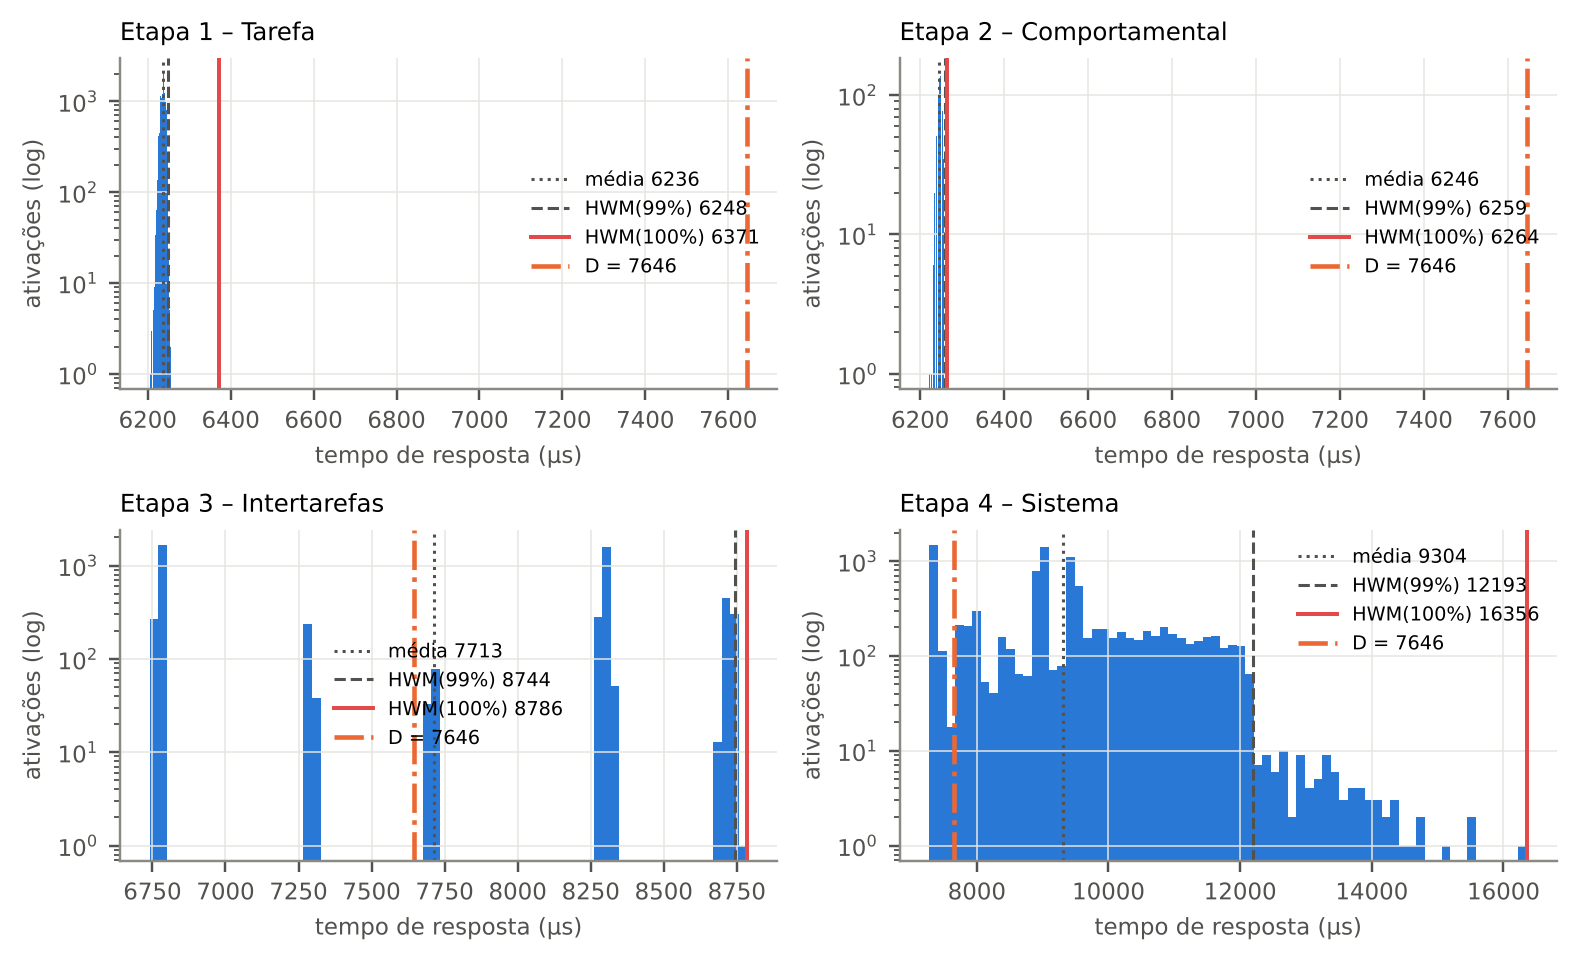
\includegraphics[width=\linewidth]{res/f_hist.png}
\caption{Histogramas (eixo vertical logarítmico) com média, HWM(99\%), HWM(100\%) e $D$.}\label{fig:hist}
\end{figure}

\subsection{Histogramas e gráficos temporais (6.2)}
\textbf{Etapa 1.} 99\% das 10\,000 medições ficam entre 6205 e 6248\,\textmu s (desvio/média de 0,1\%). A ``cauda'' é um único ponto: a ativação 0 (6371\,\textmu s, +2\%), a primeira execução, com cache frio; sem ela o máximo seria 6255\,\textmu s. \textbf{Etapa 2.} Faixa de 42\,\textmu s (6222--6264); a média sobe só 10\,\textmu s em relação à etapa 1, o custo de ISR e troca de contexto. Sem picos. Um evento por vez \emph{não} revela interferência.
\textbf{Etapa 3.} A distribuição é discreta, com cinco grupos (aprox. 6,76; 7,29; 7,7; 8,3 e 8,75\,ms), e a cauda é curta: HWM(100\%) $-$ HWM(99\%) $=42\us$. Os grupos são compatíveis com a execução da Huffman ($\approx$6,3\,ms) somada a 1--2 jobs do \emph{sensor} ($\approx$0,4\,ms) e/ou um do \emph{logger} ($\approx$1,5\,ms) que a preemptam (interpretação a partir dos tempos programados, não medida por tarefa). Os picos são \emph{periódicos}: 99,98\% dos pares de ativações separadas por 91 diferem em até 40\,\textmu s, e $91\times20\,\mathrm{ms}=1820\,\mathrm{ms}$ é o hiperperíodo. O HWM (8786\,\textmu s) ocorre na ativação 0, o instante crítico em que as três tarefas são liberadas juntas. \textbf{Etapa 4.} A maioria fica entre 7,3 e 9\,ms, mas há cauda longa e fina, até 16,4\,ms: 100 ativações (1\%) passam de 12\,193\,\textmu s e só 16 passam de 14\,ms. Os picos são \emph{agrupados} em rajadas (seção~\ref{sec:perdas}), não isolados.

\begin{figure}[H]\centering
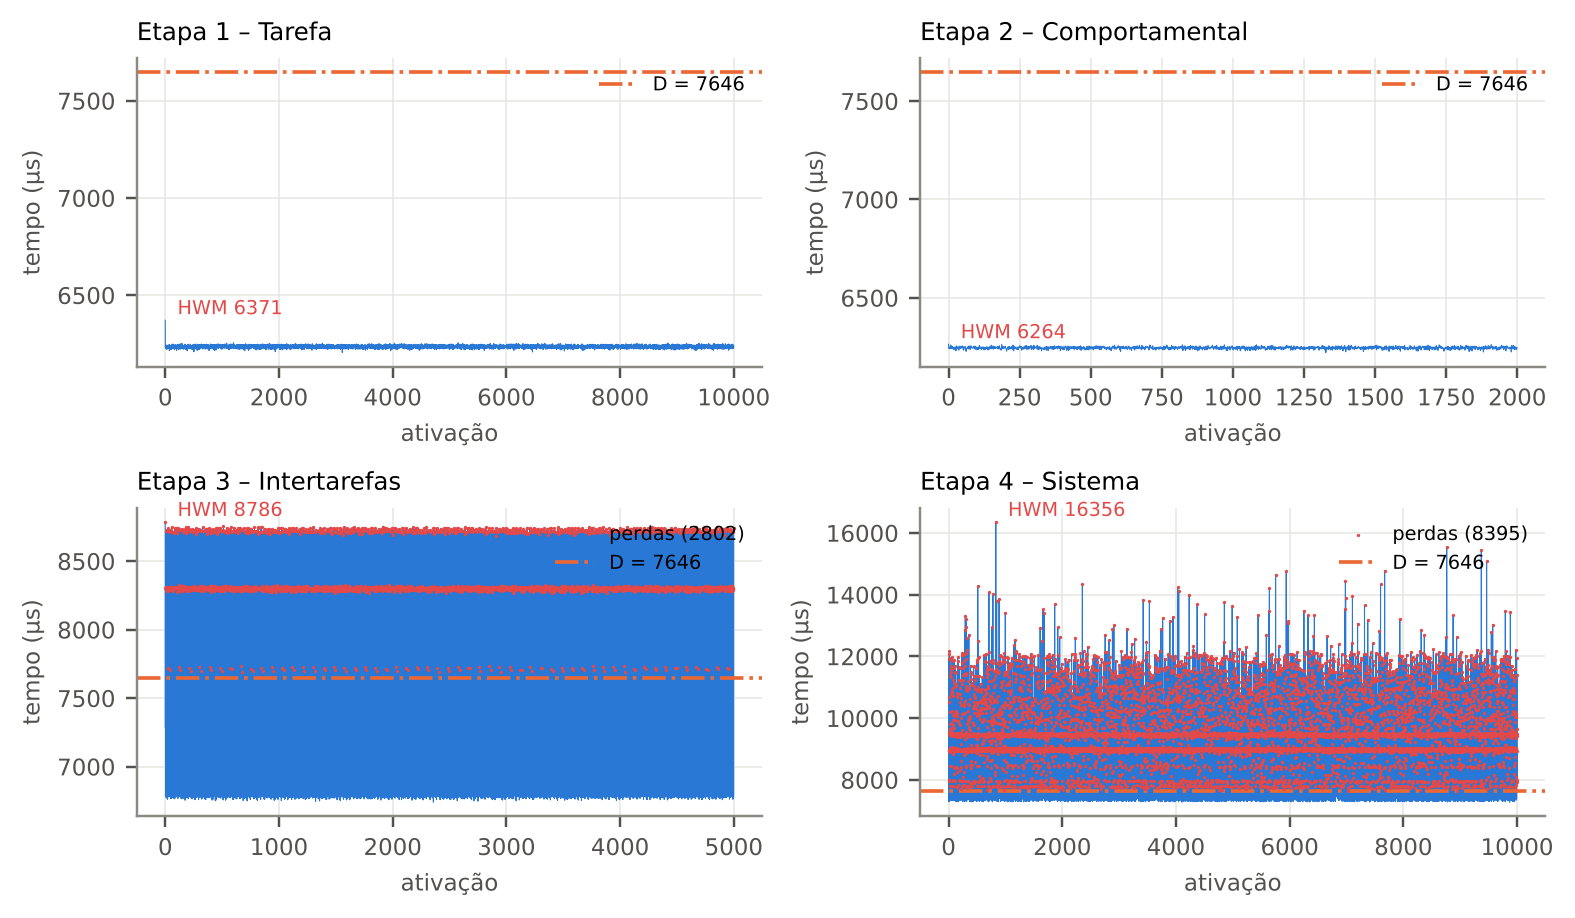
\includegraphics[width=\linewidth]{res/f_tempo.png}
\caption{Tempo de resposta $\times$ número da ativação. Pontos vermelhos: perdas de $D$; rótulo: HWM(100\%).}\label{fig:tempo}
\end{figure}

\subsection{Distâncias entre perdas e skip factor (6.3)}\label{sec:perdas}
Nas etapas 1 e 2 não houve perda. A lista completa das ativações perdidas está em \texttt{perdas\_etapa3.csv} e \texttt{perdas\_etapa4.csv} (2802 e 8395 linhas); aqui estão os começos. \textbf{Etapa 3:} ativações 0, 2, 4, 6, 8, 10, 12, 13, 15, 17, \dots; distâncias 2, 2, 2, 2, 2, 2, 1, 2, 2, 2, 2, 2, 2, 1, 1, 1, \dots \textbf{Etapa 4:} ativações 0, 1, 2, 4, 6, 8, 10, 11, 12, \dots; distâncias 1, 1, 2, 2, 2, 2, 1, 1, 1, 1, 1, 2, 2, \dots

\begin{table}[H]\centering\small
\begin{tabular}{@{}lccccccc@{}}
\toprule
\textbf{Etapa} & \textbf{Perdas} & \textbf{S} & \textbf{Dist. mediana} & \textbf{Dist. máxima} & \textbf{Isoladas} & \textbf{Rajadas ($\ge2$)} & \textbf{Maior rajada}\\\midrule
3 & 2802 & 1 & 2 & 2 & 1814 & 384 & 4\\
4 & 8395 & 1 & 1 & 2 & 640 & 966 & 38\\\bottomrule
\end{tabular}
\caption{Perdas com $D=7646\us$. Em ambas as etapas não existem duas ativações \emph{no prazo} consecutivas.}
\end{table}
Em ambas $S=1$: há perdas em ativações vizinhas. Na etapa 3 o padrão é regular (distâncias 1 ou 2, repetido a cada 91 ativações); na etapa 4 predominam distâncias 1 (81\%), com rajadas de até 38 perdas seguidas.

\subsection{Janela deslizante e (m,k)-firme (6.4)}\label{sec:mk}
\begin{figure}[H]\centering
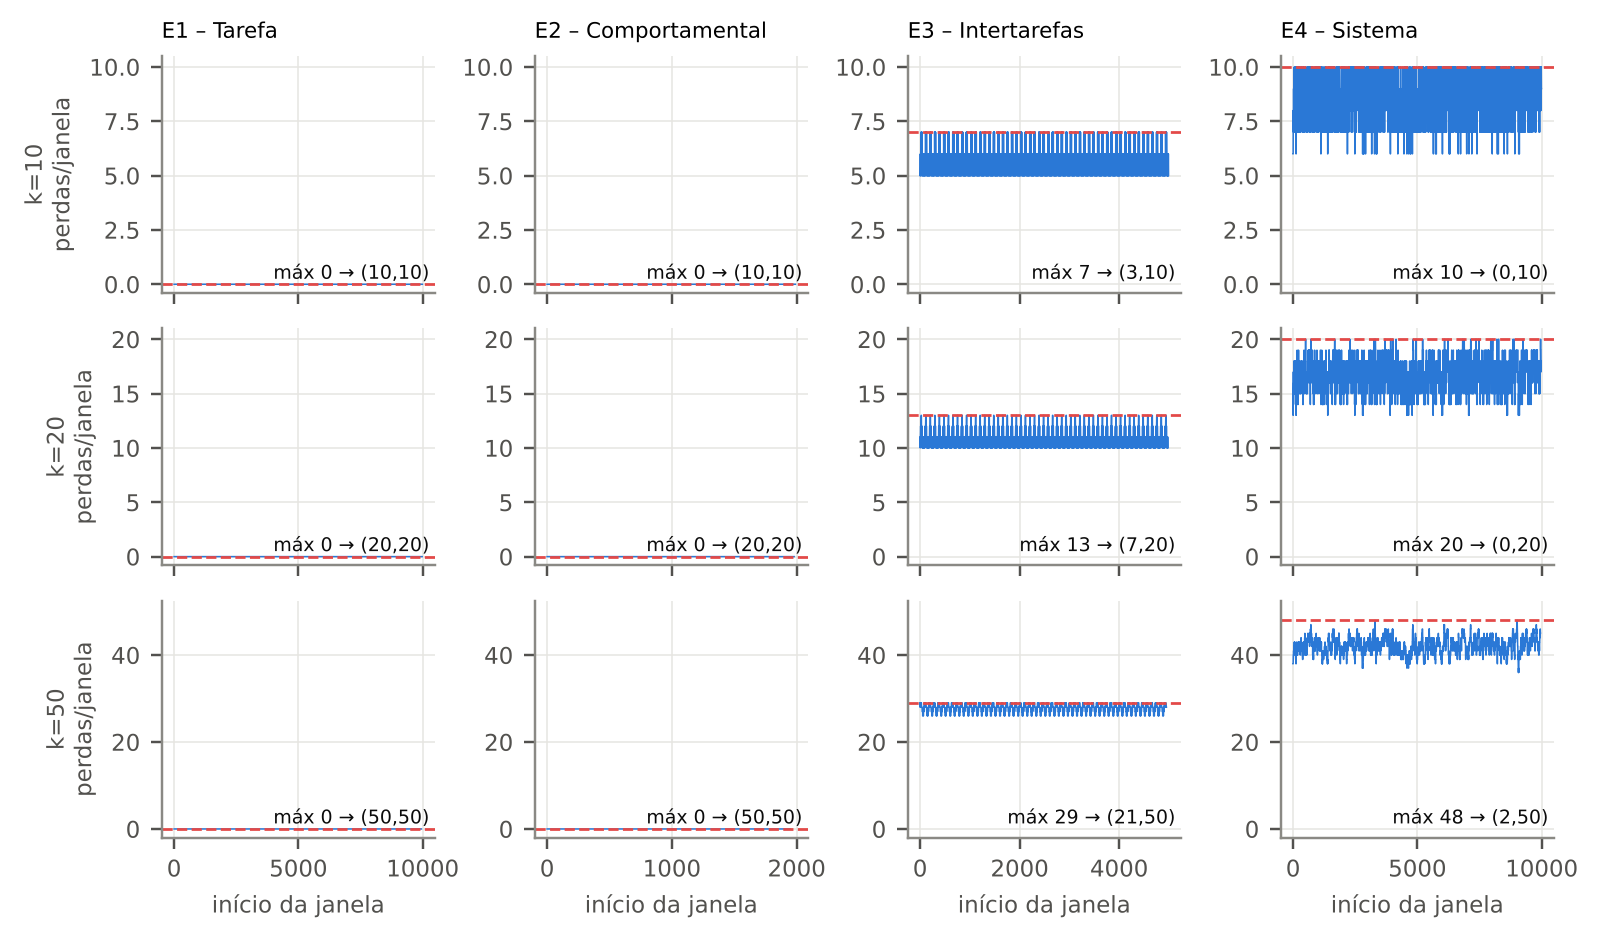
\includegraphics[width=\linewidth]{res/f_janela.png}
\caption{Deadlines perdidos por janela deslizante ($k=10,20,50$), por etapa. Linha tracejada: pior janela; $m=k-\mathrm{perdas}_{\max}$.}\label{fig:janela}
\end{figure}
Percorrendo a janela sobre toda a sequência, as etapas 1 e 2 são (10,10)-, (20,20)- e (50,50)-firmes. A etapa 3 exibe (3,10), (7,20) e (21,50): na pior janela de 20 ativações, 13 perdem o prazo (o exemplo da aula tinha 6 perdas, (14,20)). A etapa 4 exibe (0,10), (0,20) e (2,50): existem janelas de 10 e de 20 ativações \emph{sem nenhum} prazo cumprido, e a pior de 50 tem 48 perdas. Os valores da Tabela~\ref{tab:sint} são exatamente esses.

\textbf{Significado e limites.} O (m,k) obtido descreve o comportamento \emph{observado}; não é garantia formal. (i)~Uma janela pior pode existir fora da amostra: o HWM da etapa 4 ainda saltou na ativação 832 (Experimento B). (ii)~Depende do cenário: outra fase de liberação, outra carga, temperatura ou tráfego de flash diferente podem gerar janelas piores. (iii)~Janelas deslizantes se sobrepõem, logo as $\approx$10\,000 janelas não são amostras independentes. (iv)~Na etapa 3 o padrão se repete a cada hiperperíodo, o que torna o (7,20) uma propriedade estável \emph{desse} escalonamento, mas só para essa fase e esse hardware. (v)~Vale apenas para o $D$ usado (Experimento D). O (m,k) é útil como \emph{critério testável} (``sob a campanha X, nenhuma janela de 20 pode ter mais de 2 perdas''), com resultado passa/falha, mas continua sendo evidência de teste, não prova.

\section{Experimentos}
\subsection*{A. Limites da cobertura}
Com \texttt{gcov} sobre \texttt{huffman.c} (compilado no PC com \texttt{-O0 --coverage}; o fonte é o mesmo do firmware), 9 casos dirigidos (T1 entrada vazia; T2 um símbolo; T3 dois símbolos; T4 256 símbolos de mesma frequência; T5 frequências de Fibonacci/árvore degenerada; T6 2048 bytes aleatórios; T7 \emph{overflow} do buffer de bits; T8 decodificação além do fim; T9 injeção de falha na validação) atingem \textbf{100\% das 109 linhas e 100\% dos 58 desvios}, mais 11/11 chamadas, com 0 falhas. Esse é o valor da coluna ``Cobertura''.

Com a cobertura saturada, o HWM(100\%) da etapa 1 é $6371\us$. Nas outras etapas é $6264\us$ ($0{,}98\times$), $8786\us$ ($1{,}38\times$) e $16\,356\us$ ($2{,}57\times$), \emph{sem executar nenhuma linha nova}. Na campanha aleatória de 10\,000 execuções no PC (Linux, Xeon 2,1\,GHz, 2 vCPUs, ambiente de geração deste relatório; os valores mudam de máquina para máquina), o HWM foi 554,6\us em 10 e 20 amostras, 804,9\us em 100 e 3\,316\us em 1\,000, contra média de 522\us, com cobertura já em 100\%. Na ESP32 isolada o HWM da etapa 1 quase não cresce depois da ativação 0 (de 6236 a 6255\,\textmu s em 1\,200 amostras), porque a plataforma é pouco variável; o crescimento aparece quando o escopo aumenta. \emph{Conclusão:} a cobertura garante que a lógica foi exercitada e validada (\texttt{huff\_fail=0}), mas o pior tempo depende do hardware e de quando as tarefas competem; ``cobrir 100\% dos caminhos'' não encontra o WCRT.

\subsection*{B. Convergência do HWM}
\begin{minipage}[c]{0.56\linewidth}
\centering\scriptsize
\begin{tabular}{@{}lrrrrr@{}}
\toprule
\textbf{Etapa} & \textbf{10} & \textbf{20} & \textbf{100} & \textbf{1000} & \textbf{10000}\\\midrule
1 & 6371 & 6371 & 6371 & 6371 & 6371\\
2 & 6264 & 6264 & 6264 & 6264 & ---\\
3 & 8786 & 8786 & 8786 & 8786 & ---\\
4 & 11934 & 12193 & 12193 & 16356 & 16356\\\bottomrule
\end{tabular}
\captionof{table}{HWM acumulado (\textmu s) por nº de amostras.}
\end{minipage}\hfill
\begin{minipage}[c]{0.42\linewidth}
\centering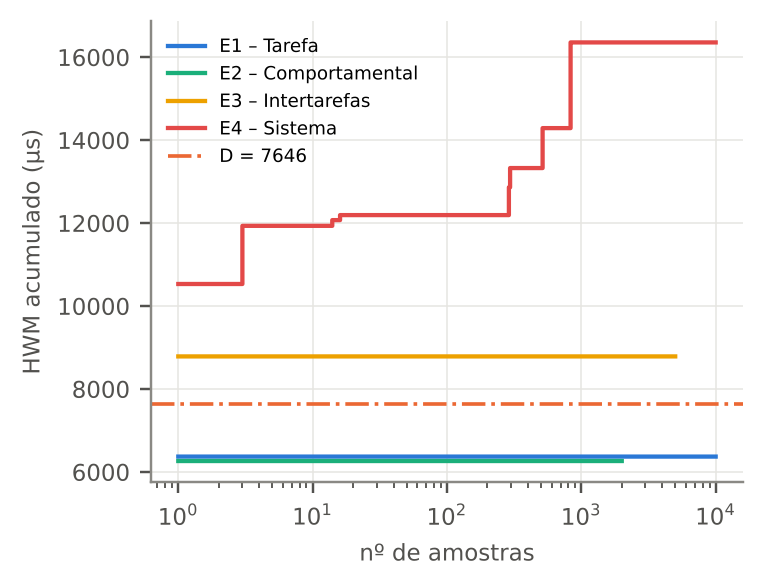
\includegraphics[width=\linewidth]{res/f_conv.png}
\captionof{figure}{Convergência do HWM.}\label{fig:conv}
\end{minipage}

Na etapa 4 o HWM saltou nas ativações 1, 3, 14, 16, 289, 295, 515 e \textbf{832} (de 12\,193 a 16\,356\,\textmu s) e não mudou nas 9\,168 seguintes: parece estabilizar perto de 1\,000 amostras, mas 10\,000 amostras não provam que não haverá novo salto. Houve \textbf{saltos tardios}. Com 10 ou 20 amostras o sistema pareceria mais rápido do que é: 27,0\% e 25,5\% abaixo do HWM final. Nas etapas 1--3 o HWM já está completo na primeira ativação, porque o pior caso (cache frio, instante crítico) está no começo, e não porque a distribuição seja estável; sem os 10\,000 pontos, não saberíamos disso.

\subsection*{C. Margem de segurança}
\begin{table}[H]\centering\small
\begin{tabular}{@{}lccccc@{}}
\toprule
\textbf{Etapa} & \textbf{HWM(100\%)} & \textbf{+10\% (7008)} & \textbf{+25\% (7964)} & \textbf{+50\% (9556)} & \textbf{Margem necessária}\\\midrule
2 & 6264 & suficiente & suficiente & suficiente & $-1{,}7\%$\\
3 & 8786 & insuficiente & insuficiente & suficiente & $+37{,}9\%$\\
4 & 16356 & insuficiente & insuficiente & insuficiente & $+156{,}7\%$\\\bottomrule
\end{tabular}
\caption{Margens sobre o HWM da etapa 1 (6371\,\textmu s), em \textmu s, comparadas com o HWM de cada etapa.}
\end{table}
A margem deixa de bastar na \textbf{etapa 3} para 10\% e 25\% (e para o próprio $D$, +20\%), e na \textbf{etapa 4} para todas, inclusive 50\%. Uma margem fixa não é adequada quando a variabilidade muda: o desvio/média vai de 0,1\% (etapas 1 e 2) a 10,3\% (etapa 3) e 14,6\% (etapa 4), e HWM/mediana de 1,02 a 1,81. Uma margem calibrada na etapa 1 \emph{herda a baixa variabilidade da etapa 1}. É o caso do exemplo da aula: uma faixa de 12--14\,ms (amplitude de 2\,ms) que passa a 10--16\,ms (6\,ms) triplica a amplitude, e a margem escolhida na primeira faixa deixa de cobrir a segunda. A margem deve ser derivada da variabilidade medida no escopo mais amplo.

\subsection*{D. Perdas e (m,k)-firme sob diferentes deadlines}
Usamos $D_1=\mathrm{HWM}_{100\%}^{(1)}=6371$, $D_{fixo}=7646$, o intermediário $D_3=9282$, $D_4=\mathrm{HWM}_{99\%}^{(4)}=12193$ e $D_5=\mathrm{HWM}_{100\%}^{(4)}=16356$.
\begin{table}[H]\centering\scriptsize
\setlength{\tabcolsep}{3.8pt}
\begin{tabular}{@{}cr rrrc rrr@{}}
\toprule
\textbf{Etapa} & \textbf{D (\textmu s)} & \textbf{\% cumprido} & \textbf{Perdas} & \textbf{S} & \textbf{(m,20)} & \textbf{Isoladas} & \textbf{Rajadas} & \textbf{Maior}\\\midrule
3 & 6371 & 0,00 & 5000 & 1 & (0,20) & 0 & 1 & 5000\\
3 & 7646 & 43,96 & 2802 & 1 & (7,20) & 1814 & 384 & 4\\
3 & 9282 / 12193 / 16356 & 100,00 & 0 & --- & (20,20) & 0 & 0 & 0\\\midrule
4 & 6371 & 0,00 & 10000 & 1 & (0,20) & 0 & 1 & 10000\\
4 & 7646 & 16,05 & 8395 & 1 & (0,20) & 640 & 966 & 38\\
4 & 9282 & 51,19 & 4881 & 1 & (4,20) & 1734 & 1019 & 8\\
4 & 12193 & 99,00 & 100 & 4 & (17,20) & 100 & 0 & 1\\
4 & 16356 & 100,00 & 0 & --- & (20,20) & 0 & 0 & 0\\\bottomrule
\end{tabular}
\caption{Análises 6.3 e 6.4 para vários $D$ (k=20). Com $D_1$ todas as ativações são perdas: uma rajada única.}\label{tab:expd}
\end{table}
\textbf{Menor $D$ para um (m,k) exigido (etapa 4, k=20).} (10,20): $10\,548\us$ (64,5\% do HWM da etapa 4); (14,20): $11\,639\us$ (71,2\%); \textbf{(18,20): $13\,533\us$ (82,7\%)}; (19,20): $14\,114\us$ (86,3\%); (20,20): $16\,356\us$ (100\%, o próprio HWM). Exigir (18,20) permite um $D$ 2\,823\,\textmu s (17,3\%) menor que $D=\mathrm{HWM}_{100\%}$, com 99,72\% de ativações no prazo. Note que $D_4=\mathrm{HWM}_{99\%}$ (99\% no prazo) dá só (17,20), e não (18,20): três perdas isoladas podem caber numa mesma janela de 20, de modo que \emph{percentual alto não implica (m,k) alto}.

\textbf{Isoladas $\times$ rajadas.} Com $D_{fixo}$ a etapa 4 tem rajadas de até 38 perdas seguidas; com $D_3$, até 8; com $D_4$, as 100 perdas são todas isoladas (distância mediana 66, máxima 442). Para um sistema com inércia física (como o motor de primeira ordem da esteira do M2), uma perda isolada é filtrada: a planta não responde em uma ativação, e a seguinte corrige o erro. Uma rajada acumula atraso além do que a inércia absorve. Por isso o que importa é o tempo entre perdas consecutivas e não só o percentual: 1\% de perdas espalhadas é (17,20), mas as mesmas 100 perdas num bloco único dariam janelas (0,20).

\begin{figure}[H]\centering
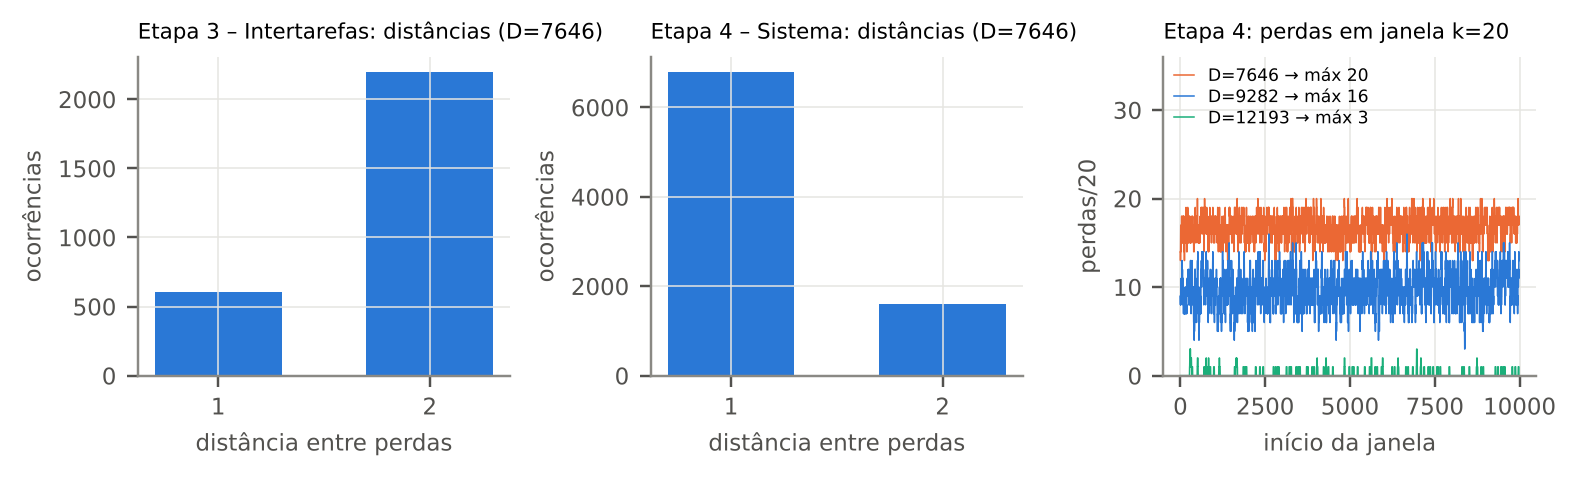
\includegraphics[width=0.86\linewidth]{res/f_dist.png}
\caption{Distâncias entre perdas (etapas 3 e 4, $D=7646\us$) e perdas em janela k=20 na etapa 4 para três valores de $D$.}\label{fig:dist}
\end{figure}

\section{Ameaças à validade}
\begin{itemize}
\item \textbf{Plataforma de propósito geral.} A flash e o barramento são compartilhados entre os dois núcleos, e ISRs do SDK e o tick de 1\,kHz interferem; os resultados valem para esta placa, este firmware e esta versão do IDF.
\item \textbf{Estados ocultos de cache e energia.} A ativação 0 (cache frio) vale +2\% na etapa 1 e define o HWM e o $D$. A frequência é fixa e não há DFS, mas a temperatura não foi controlada.
\item \textbf{Interrupções do SO.} Não foram isoladas: estão dentro das medições, mas a taxa em que ocorrem é desconhecida.
\item \textbf{Efeito da instrumentação.} A leitura do relógio e a escrita do vetor somam microssegundos; o desvio entre relógios foi corrigido com janela de calibração de 2\,\textmu s, logo as etapas 2--4 têm incerteza da ordem de $\pm2\us$. O primeiro escopo mede execução e os demais, liberação$\to$conclusão, o que é proposital mas muda a métrica.
\item \textbf{Cenários de estresse não cobertos.} Wi-Fi/Bluetooth, outras fases de liberação, taxas de interrupção maiores e padrões de acesso à flash diferentes. Uma execução por etapa, sem repetição nem intervalo de confiança. A cobertura foi medida no PC (x86, \texttt{-O0}), não no ESP32.
\item \textbf{Escolha de $D$.} $D=1{,}2\times$HWM da etapa 1 ($7646\us$) está abaixo da média da etapa 3 ($7713\us$); a taxa de perda das etapas 3 e 4 reflete esse $D$, não uma falha de projeto da Huffman.
\end{itemize}

\section{Conclusão}
Medir só a tarefa isolada (etapa 1) ou com um evento por vez (etapa 2) diria que o sistema é rápido e previsível (6,2\,ms, 100\% no prazo), com cobertura de 100\% de linha e de desvio. No escopo intertarefas o HWM sobe 38\% e, no de sistema, 157\%, com 56\% e 84\% de perdas para o mesmo $D$. Isso responde à primeira pergunta: a cobertura valida a \emph{lógica}, mas o WCRT depende de preempção, bloqueio, interrupções e barramento, que só aparecem nos escopos maiores, e o HWM continua mudando (salto na ativação 832 da etapa 4) enquanto a cobertura não muda. Quando o WCRT não é alcançável, o (m,k)-firme por janela deslizante converte as medições em um critério verificável: no sistema completo, (18,20) exige $D\ge13\,533\us$ (17\% abaixo do HWM) e o HWM(99\%) sozinho já não basta. O (m,k) medido é \emph{observação}, não garantia: a margem e o $D$ precisam derivar da variabilidade medida no escopo de sistema, e qualquer valor deve vir acompanhado da campanha e da carga que o produziram.

\noindent\textbf{Reprodução.}
\begin{itemize}\footnotesize
\item \texttt{idf.py set-target esp32; idf.py build flash}
\item \texttt{python tools/capture.py --port /dev/ttyUSB0 --baud 921600 --out data; ./host/run\_coverage.sh}
\item \texttt{python analysis/analyze.py --data data --out results --cov-line 100 --cov-branch 100 --mk-required 18,20}
\item \texttt{python relatorio\_analise.py --repo . --out res}
\end{itemize}
\end{document}
